\documentclass[10pt]{article}
\usepackage{pgf,tikz,pgfplots}
\pgfplotsset{compat=1.15}
\usepackage{mathrsfs}
\usetikzlibrary{arrows}
\usepackage{listings}
\usepackage{etoolbox}
\pagestyle{empty}
\BeforeBeginEnvironment{lstlisting}{\par\noindent\begin{minipage}{\linewidth}}
\AfterEndEnvironment{lstlisting}{\end{minipage}\par\addvspace{\topskip}}

\begin{document}

\definecolor{rvwvcq}{rgb}{0.08235294117647059,0.396078431372549,0.7529411764705882}
\begin{lstlisting}[numbers=left,numbersep=5pt,mathescape=true,caption=Refinement of transactions (dealing with task completion),label=lst:nrefine2]
handleTaskCompletion(CompensatableTask c, BPMN2Process p) {
  // A send message event to indicate the task is done
  Event doneSendEvent = new SendMessagEvent();
  // A receive message event to catch the message above
  Event doneReceiveEvent = new ReceiveMessageEvent();  
  doneSendEvent.receivers = {doneReceiveEvent};
  // Placing the message event after the task
  if (c.nextFlowObjects == null) {
    c.nextFlowObjects = {doneSendEvent};
  } else {
    Gateway gf = new ForkGateway();
    gf.nextFlowObjects = c.nextFlowObjects;
    gf.nextFlowObjects.add(doneSendEvent);
    c.nextFlowObjects = {gf};
  }
}
\end{lstlisting}
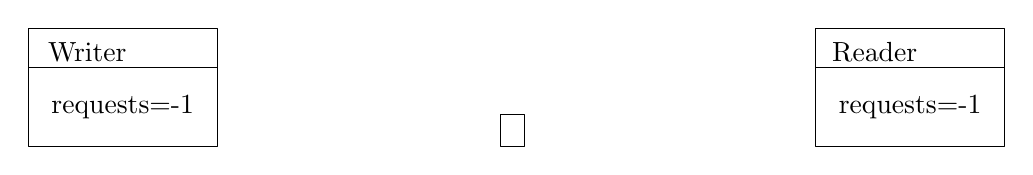
\begin{tikzpicture}[line cap=round,line join=round,>=triangle 45,x=1cm,y=1cm]
(15.129269413933608,6.743153952022232);
\fill[white, draw=black] (0,4.5) rectangle (2.4,5.5);
\fill[white, draw=black] (0,4) rectangle (2.4,5);
\draw (1.2,4.5) node {requests=-1};
\draw (.75,5.2) node {Writer};
\fill[white, draw=black] (6,4) rectangle (6.3,4.4);
\fill[white, draw=black] (10,4.5) rectangle (12.4,5.5);
\fill[white, draw=black] (10,4) rectangle (12.4,5);
\draw (11.2,4.5) node {requests=-1};
\draw (10.75,5.2) node {Reader};
\end{tikzpicture}
\newpage
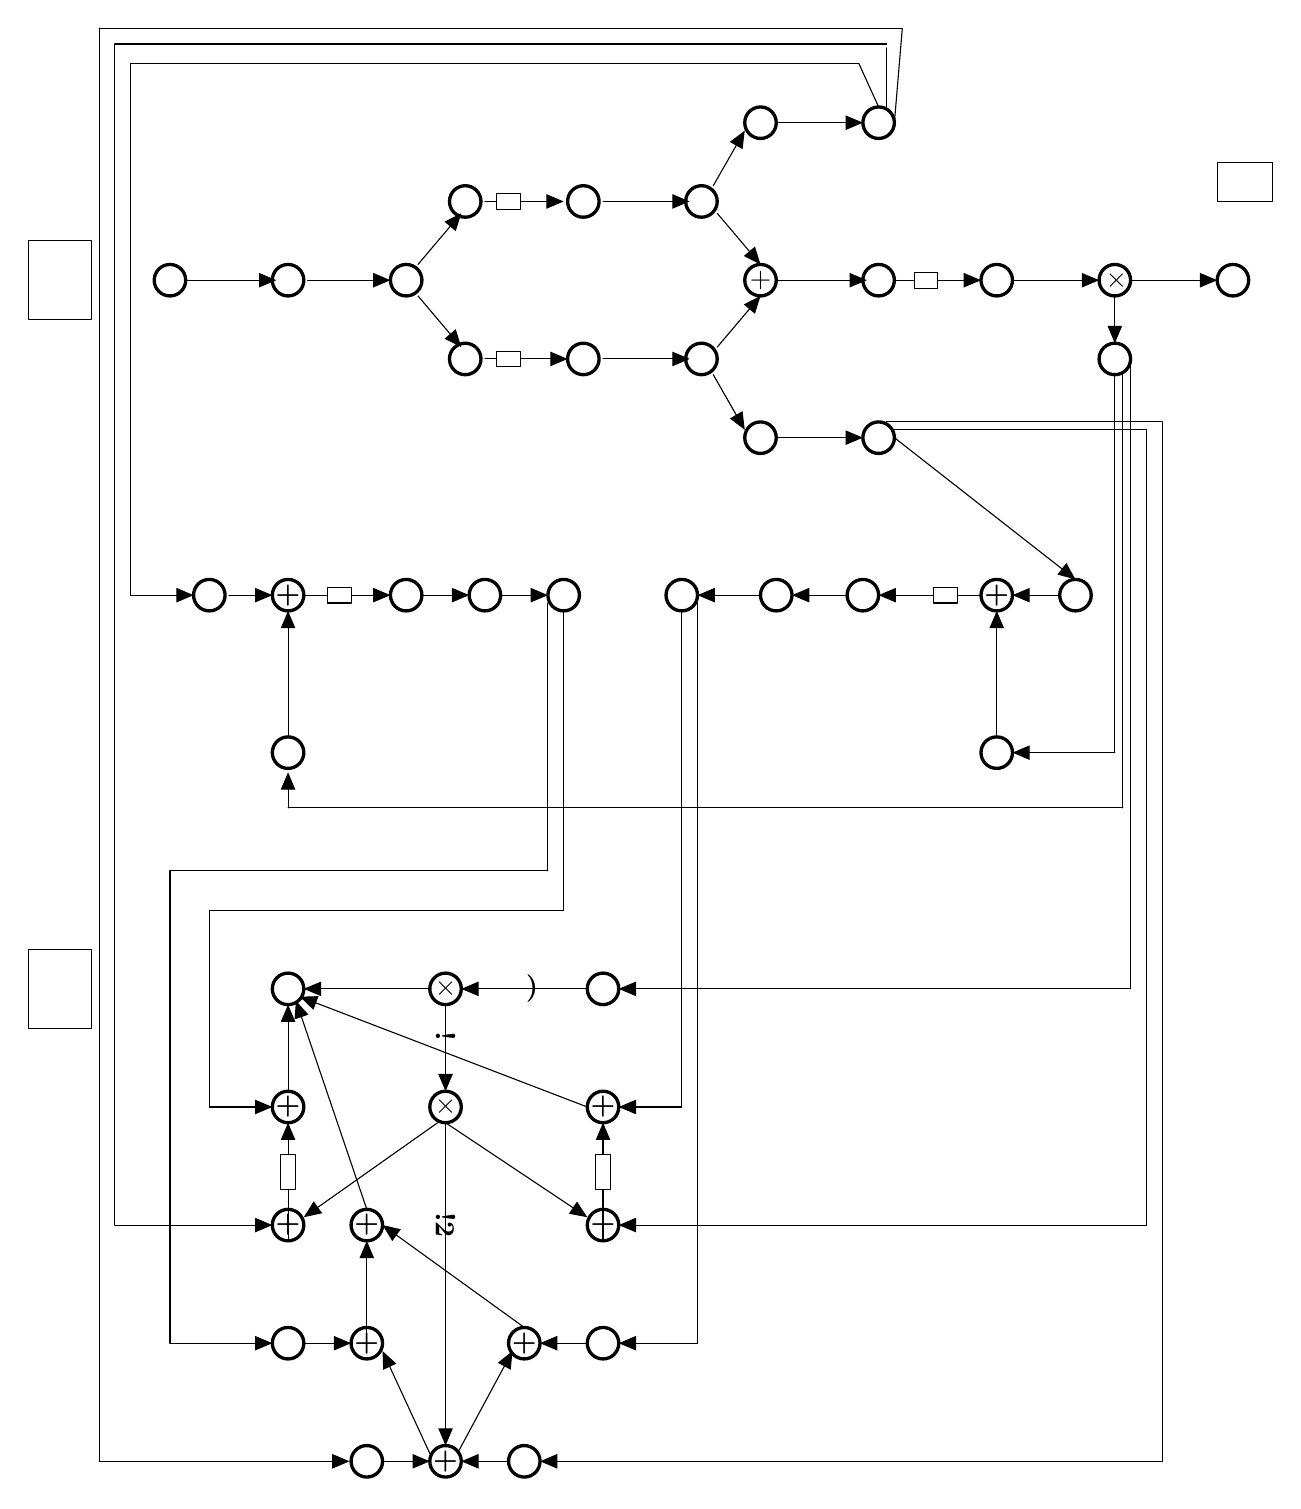
\begin{tikzpicture}[line cap=round,line join=round,>=triangle 45,x=1cm,y=1cm]
%%sings
\draw (2,-9) node {$\times$};
\draw (2,-10.5) node {$\times$};
\draw (0,-4) node {\textbf{+}};
\draw (9,-4) node {\textbf{+}};
\draw (3.1,-9) node {\textbf{)}};
\draw (0,-12) node {\textbf{+}};
\draw (1,-12) node {\textbf{+}};
\draw (4,-12) node {\textbf{+}};
\draw (0,-10.5) node {\textbf{+}};
\draw (4,-10.5) node {\textbf{+}};
\draw (2,-15) node {\textbf{+}};
\draw (1,-13.5) node {\textbf{+}};
\draw (3,-13.5) node {\textbf{+}};
\node[rotate=-90] at (2, -9.6) (b) {\textbf{!}};%%priority
\node[rotate=-90] at (2, -12) (b) {\textbf{!2}};%%priority
%%%%
\draw [line width=1.2pt] (-.75*2,0) circle (0.2cm);
\draw [line width=1.2pt] (0,0) circle (0.2cm);
\draw [line width=1.2pt] (.75*2,0) circle (0.2cm);
\draw [line width=1.2pt] (.75*3,1) circle (0.2cm);
\draw [line width=1.2pt] (.75*3,-1) circle (0.2cm);
\draw [line width=1.2pt] (.75*5,-1) circle (0.2cm);
\draw [line width=1.2pt] (.75*5,1) circle (0.2cm);
\draw [line width=1.2pt] (.75*7,1) circle (0.2cm);
\draw [line width=1.2pt] (.75*7,-1) circle (0.2cm);
\draw [line width=1.2pt] (.75*8,0) circle (0.2cm);
\draw [line width=1.2pt] (.75*10,0) circle (0.2cm);
\draw [line width=1.2pt] (.75*12,0) circle (0.2cm);
\draw [line width=1.2pt] (.75*14,0) circle (0.2cm);
\draw [line width=1.2pt] (.75*16,0) circle (0.2cm);
\draw [line width=1.2pt] (.75*14,-1) circle (0.2cm);
%%%%%%%%%%%%%%%%%
\draw [line width=1.2pt] (.75*8,2) circle (0.2cm);%highest
\draw [line width=1.2pt] (.75*8,-2) circle (0.2cm);
\draw [line width=1.2pt] (7.5,2) circle (0.2cm);%highest
\draw [line width=1.2pt] (.75*10,-2) circle (0.2cm);
%%%%%%
\draw [->] (0.75*-1.75,0) -- (-.15,0);
\draw [->] (0.25,0) -- (1.3,0);
\draw [->] (1.65,.2) -- (2.2,.85);
\draw [->] (1.65,-.2) -- (2.2,-.85);
\draw [->] (4, 1) -- (5.1,1);
\draw [->] (4,-1) -- (5.1,-1);
\draw [->] (5.45,.85) -- (6,.2);
\draw (6,0) node {+};
\draw [->] (5.45,-.85) -- (6,-.2);%%%
\draw [->] (6.2, 0) -- (7.35,0);
\draw [->] (7.7, 0) -- (8.8,0);
\draw [->] (9.2, 0) -- (10.3,0);
\draw [->] (10.7, 0) -- (11.8,0);
\draw (10.52,0) node {$\times$};
\draw [->] (10.5, -.2) -- (10.5,-.8);
%%% upper layer
\draw [->] (5.4,1.2) -- (5.8,1.9);%
\draw [->] (6.2,2) -- (7.3,2);
\draw [->] (2.5,1) -- (3.5,1);
\draw [->] (2.5,-1) -- (3.55,-1);
%%% lower layer
\draw [->] (5.4,-1.2) -- (5.8,-1.9);%
\draw [->] (6.2,-2) -- (7.3,-2);
%%%%%%Undo part
\draw [line width=1.2pt] (-1,-4) circle (0.2cm);%
\draw [line width=1.2pt] (0,-4) circle (0.2cm);%
\draw [line width=1.2pt] (1.5,-4) circle (0.2cm);%
\draw [line width=1.2pt] (2.5,-4) circle (0.2cm);%
\draw [line width=1.2pt] (3.5,-4) circle (0.2cm);%
\draw [line width=1.2pt] (0,-6) circle (0.2cm);%
\draw [->] (-.75,-4) -- (-.2,-4);%flight undo
\draw [->] (.2,-4) -- (1.3,-4);%fifo
\draw [->] (1.7,-4) -- (2.3,-4);
\draw [->] (2.7,-4) -- (3.3,-4);
%%amoodi
\draw [->] (9,-5.8) -- (9,-4.2);
%undo part 2
\draw [line width=1.2pt] (10,-4) circle (0.2cm);%
\draw [line width=1.2pt] (9,-4) circle (0.2cm);%
\draw [line width=1.2pt] (7.3,-4) circle (0.2cm);%
\draw [line width=1.2pt] (6.2,-4) circle (0.2cm);%
\draw [line width=1.2pt] (5,-4) circle (0.2cm);%
\draw [line width=1.2pt] (9,-6) circle (0.2cm);%
\draw [->] (9.8,-4) -- (9.2,-4);
\draw [->] (8.8,-4) -- (7.5,-4);
\draw [->] (7.1,-4) -- (6.4,-4);
\draw [->] (6,-4) -- (5.2,-4);
%%amoodi
\draw [->] (0,-5.8) -- (0,-4.2);
%%%%%%cancel part
\draw [line width=1.2pt] (0,-9) circle (0.2cm);%r1
\draw [line width=1.2pt] (2,-9) circle (0.2cm);%r1
\draw [line width=1.2pt] (4,-9) circle (0.2cm);%r1
\draw [->] (1.8,-9) -- (.2,-9);%
\draw [->] (3.8,-9) -- (2.2,-9);%
\draw [->] (2,-9.2) -- (2,-10.3);%
%%
\draw [line width=1.2pt] (2,-10.5) circle (0.2cm);%r2
\draw [line width=1.2pt] (4,-10.5) circle (0.2cm);%r2
%\draw [->] (1.9,-10.7) -- (1,-11.23);%left
%\draw [->] (0,-11.8) -- (1,-11.23);%left
\draw [<-] (.2,-11.9) -- (1.9,-10.7);%left
%\draw [->] (2,-10.7) -- (3,-11.27);%right
%\draw [->] (4,-11.8) -- (3,-11.27);%right
\draw [->] (2,-10.7) -- (3.8,-11.9);%right
%\draw [-] (2,-10.7) -- (2,-11.4);%inner cancel next
\draw [->] (2,-10.7) -- (2,-14.8);%inner cancel next
\draw [->] (0,-10.3) -- (0,-9.2);%finish
%%
\draw [line width=1.2pt] (0,-12) circle (0.2cm);%r3
%\draw [line width=1.2pt] (2,-12) circle (0.2cm);%r3
\draw [line width=1.2pt] (4,-12) circle (0.2cm);%r3
\draw [->] (0,-12.2) -- (0,-10.7);%amoodi
%\draw [<-] (2,-12.2) -- (2,-14.8);%amoodi
\draw [->] (4,-12.2) -- (4,-10.7);%amoodi
\draw [<-] (3.2,-13.5) -- (3.8,-13.5);%horiz
\draw [<-] (.8,-13.5) -- (.2,-13.5);%horiz
\draw [<-] (1.2,-13.6) -- (1.8,-14.9);%kaj
\draw [<-] (2.85,-13.6) -- (2.15,-14.9);%kaj
%r4
\draw [line width=1.2pt] (0,-10.5) circle (0.2cm);%r4
\draw [line width=1.2pt] (4,-13.5) circle (0.2cm);%r4
\draw [line width=1.2pt] (0,-13.5) circle (0.2cm);%r4both compensation 
\draw [line width=1.2pt] (1,-13.5) circle (0.2cm);%r4both
\draw [line width=1.2pt] (3,-13.5) circle (0.2cm);%r4both
\draw [<-] (1.8,-15) -- (1.2,-15);%horiz
\draw [<-] (2.2,-15) -- (2.8,-15);%horiz
%%r4.5
\draw [line width=1.2pt] (1,-12) circle (0.2cm);%r4
\draw [<-] (1,-12.2) -- (1,-13.5);
\draw [->] (3,-13.3) -- (1.2,-12);
\draw [<-] (.1,-9.15) -- (1,-11.8);%finish
\draw [<-] (.15,-9.1) -- (3.8,-10.5);%finish
%r5
\draw [line width=1.2pt] (1,-15) circle (0.2cm);%r5
\draw [line width=1.2pt] (3,-15) circle (0.2cm);%r5
\draw [line width=1.2pt] (2,-15) circle (0.2cm);%r4
%%%Done hotel to others
\draw [-] (7.5,2.2) -- (7.25,2.75);
\draw [-] (7.25, 2.75) -- (-2, 2.75);
\draw [-] (7.25, 2.75) -- (-1.5, 2.75);
\draw [-] (-2, 2.75) -- (-2, -4);
\draw [->] (-2, -4) -- (-1.2, -4);
%%%Done hotel to end
\draw [-] (7.6,2.2) -- (7.6,2.949);
\draw [-] (7.6, 3) -- (-2.2, 3);
\draw [-] (7.6, 3) -- (-1.5, 3);
\draw [-] (-2.2, 3) -- (-2.2, -12);
\draw [->] (-2.2, -12) -- (-.2, -12);
%%%Done hotel to end both
\draw [-] (7.7,2) -- (7.8,3.19);
\draw [-] (7.8, 3.2) -- (-2.4, 3.2);
\draw [-] (7.6, 3.2) -- (-1.5, 3.2);
\draw [-] (-2.4, 3.2) -- (-2.4, -15);
\draw [->] (-2.4, -15) -- (.78, -15);
%%%Done flight to others
\draw [->] (7.7,-2) -- (10, -3.8);
%%%Done flight to both
\draw [-] (7.6,-1.8) -- (11.1,-1.8);
\draw [-] (11.1,-1.8) -- (11.1,-15);
\draw [->] (11.1, -15) -- (3.2, -15);
%%%Done fly to end
\draw [-] (10.9,-1.9) -- (7.7,-1.9);
\draw [-] (10.9,-1.9) -- (10.9,-12);
\draw [->] (10.9, -12) -- (4.2, -12);
%%Cancel to others
\draw [-] (10.5, -1.2) -- (10.5, -6);
\draw [->] (10.5, -6) -- (9.2, -6);
%%flight
\draw [-] (10.6, -1.2) -- (10.6, -6.7);
\draw [-] (10.6, -6.7) -- (0, -6.7);
\draw [->] (0, -6.7) -- (0, -6.25);
%both
\draw [-] (10.7, -1) -- (10.7, -9);
\draw [->] (10.7, -9) -- (4.2, -9);
%compensation hotel to end
\draw [-] (3.5, -4.2) -- (3.5, -8);
\draw [-] (3.5, -8) -- (-1, -8);
\draw [-] (-1, -8) -- (-1, -10.5);
\draw [->] (-1, -10.5) -- (-.2, -10.5);
%%%%%compensation hotel to both
\draw [-] (3.3, -4.1) -- (3.3, -7.5);
\draw [-] (3.3, -7.5) -- (-1.5, -7.5);
\draw [-] (-1.5, -7.5) -- (-1.5, -13.5);
\draw [->] (-1.5, -13.5) -- (-.2, -13.5);
%compensation flight to end
\draw [-] (5, -4.2) -- (5, -10.5);
\draw [->] (5, -10.5) -- (4.2, -10.5);
%%%%%compensation flight to both
\draw [-] (5.2, -4.1) -- (5.2, -13.5);
\draw [->] (5.2, -13.5) -- (4.2, -13.5);
%%%%fifos
\fill[white, draw=black] (2.65,1.1) rectangle (2.95,.9);
\fill[white, draw=black] (2.65,-1.1) rectangle (2.95,-.9);
\fill[white, draw=black] (7.95,.1) rectangle (8.25,-.1);
\fill[white, draw=black] (.5,-4.1) rectangle (.8,-3.9);
\fill[white, draw=black] (8.5,-4.1) rectangle (8.2,-3.9);
%cancel
\fill[white, draw=black] (-.1,-11.1) rectangle (.1,-11.55);%left
\fill[white, draw=black] (3.9,-11.1) rectangle (4.1,-11.55);%rightt
%ios
\fill[white, draw=black] (-3.3,-8.5) rectangle (-2.5,-9.5);%reader
\fill[white, draw=black] (-3.3,.5) rectangle (-2.5,-.5);%writer
\fill[white, draw=black] (11.8,1.5) rectangle (12.5,1);%writer
\end{tikzpicture}


\newpage
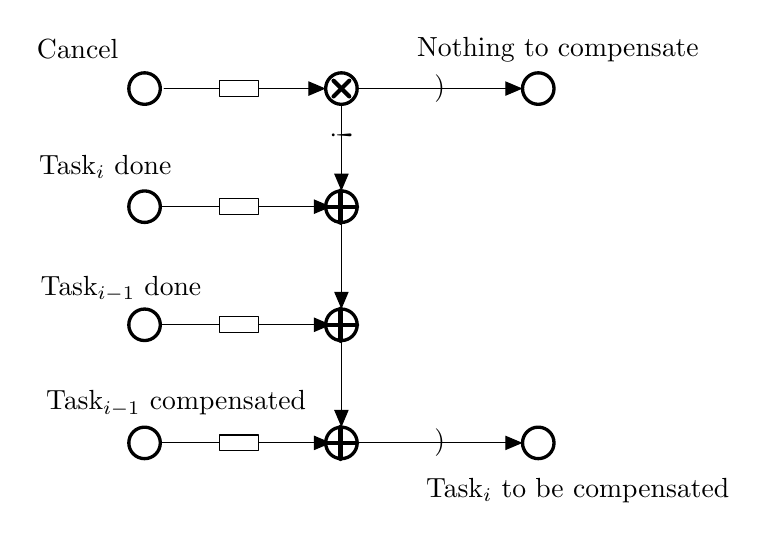
\begin{tikzpicture}[line cap=round,line join=round,>=triangle 45,x=1cm,y=1cm]
%labels
    \node[rotate=-90] at (1, -.6)   (b) {!};
    \node[] at (2.25, 0)   (b) {)};
    \node[] at (2.25, -4.5)   (b) {)};
    \node[] at (-2.35, .5)   (b) {Cancel};
    \node[] at (-2, -1)   (b) {Task$_i$ done};
    \node[] at (-1.8, -2.55)   (b) {Task$_{i-1}$ done};
    \node[] at (-1.1, -4)   (b) {Task$_{i-1}$ compensated};
    \node[] at (3.75, .5)   (b) {Nothing to compensate};
    \node[] at (4, -5.1)   (b) {Task$_i$ to be compensated};
%%%%%%%%
\draw [line width=1.2pt] (-.75*2,0) circle (0.2cm);%xel
\draw [line width=1.2pt] (.5*2,0) circle (0.2cm);%X
\draw [line width=1.2pt] (-.75*2,-1.5) circle (0.2cm);%done
\draw [line width=1.2pt] (-.75*2,-3) circle (0.2cm);%predone
\draw [line width=1.2pt] (-.75*2,-4.5) circle (0.2cm);%preundone
\draw [line width=1.2pt] (1.75*2,0) circle (0.2cm);%no compensation needed
%%%%col2
%done
\draw [line width=1.2pt] (2.5-.75*2,-3) circle (0.2cm);%predone
\draw [line width=1.2pt] (2.5-.75*2,-4.5) circle (0.2cm);%preundone
\draw [line width=1.2pt] (2.5-.75*2,-1.5) circle (0.2cm);%xel
%%%+ 3
\draw [line width=1.8pt] (.99, -3.2) -- (.99,-2.8);
\draw [line width=1.5pt] (.82, -3) -- (1.2,-3);
%%%+ 2
\draw [line width=1.8pt] (.99, -4.7) -- (.99,-4.3);
\draw [line width=1.5pt] (.82, -4.5) -- (1.2,-4.5);
%%%+ 1
\draw [line width=1.8pt] (.99, -1.7) -- (.99,-1.3);
\draw [line width=1.5pt] (.82, -1.5) -- (1.2,-1.5);
%%col3
\draw [line width=1.2pt] (5-.75*2,-4.5) circle (0.2cm);%+el 3
%%%X
\draw [line width=1.5pt] (.9, -.1) -- (1.1,.1);
\draw [line width=1.5pt] (.9, .1) -- (1.1,-.1);
%%%lines1
\draw [->] (-1.25,0) -- (.8,0);%1 cancel to X
\draw [->] (-1.3,-1.5) -- (.87,-1.5);%2
\draw [->] (-1.3,-3) -- (.87,-3);%3
\draw [->] (-1.3,-4.5) -- (.87,-4.5);%4
\draw [->] (1.2,0) -- (3.3,0);%adiiii ni compensation needed
%% X to + amoodi
\draw [->] (1,-.2) -- (1,-1.3);%2
%% khali to + 
\draw [->] (1.2,-4.5) -- (3.3,-4.5);%3ifo
%fifo
\fill[white, draw=black] (-.55,.1) rectangle (-.05,-.1);%fifo balatarintar
\fill[white, draw=black] (-.55,-1.4) rectangle (-.05,-1.6);%fifo balatarin
\fill[white, draw=black] (-.55,-2.9) rectangle (-.05,-3.1);%fifo bala
\fill[white, draw=black] (-.55,-4.4) rectangle (-.05,-4.6);%fifo paiin
%%line 2 to three
\draw [->] (1,-1.7) -- (1,-2.8);
%%line 3 to four
\draw [->] (1,-3.2) -- (1,-4.3);
\end{tikzpicture}
\newpage



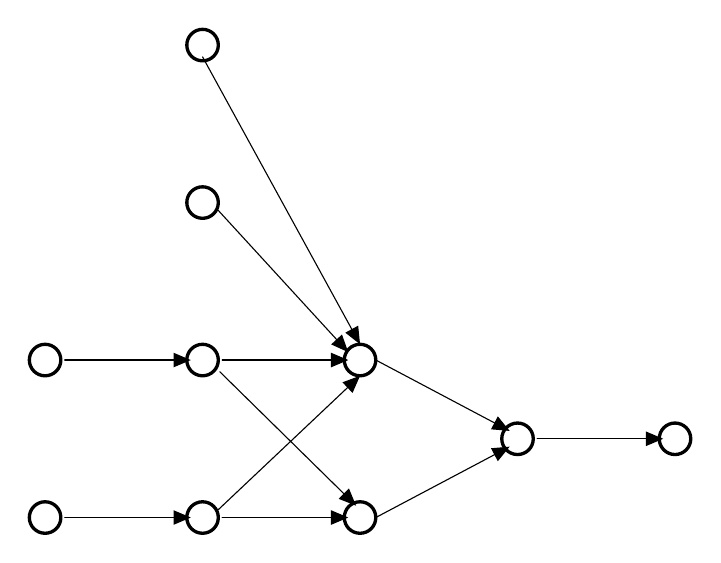
\begin{tikzpicture}[line cap=round,line join=round,>=triangle 45,x=1cm,y=1cm]

%\clip(-14.734939415430144,-11.199700639958023) rectangle (15.129269413933608,6.743153952022232);
\draw [line width=1.2pt] (0,0) circle (0.2cm);
\draw [line width=1.2pt] (0,-2) circle (0.2cm);
\draw [line width=1.2pt] (2,0) circle (0.2cm);
\draw [line width=1.2pt] (4,0) circle (0.2cm);
\draw [line width=1.2pt] (4,-2) circle (0.2cm);
\draw [line width=1.2pt] (6,-1) circle (0.2cm);
\draw [line width=1.2pt] (8,-1) circle (0.2cm);
\draw [line width=1.2pt] (2,-2) circle (0.2cm);
\draw [line width=1.2pt] (2,2) circle (0.2cm);
\draw [line width=1.2pt] (2,4) circle (0.2cm);
\draw [->] (0.25,0) -- (1.85,0);
\draw [->] (2.25,0) -- (3.85,0);
\draw [->] (2.25,-2) -- (3.85,-2);
\draw [->] (0.25,-2) -- (1.85,-2);
\draw [->] (6.25,-1) -- (7.85,-1);
%%%
\draw [->] (2,3.85) -- (4,0.2);
\draw [->] (2.2,1.9) -- (3.85,0.1);
%%
\draw [->] (2.22,-.15) -- (3.95,-1.85);
\draw [->] (2.2,-1.9) -- (4,-.2);
%%
\draw [->] (4.2,0) -- (5.9,-.9);
\draw [->] (4.2,-2) -- (5.9,-1.1);
%%
\end{tikzpicture}
\end{document}
